\documentclass[border=10pt]{standalone}

\usepackage{tikz}
\usepackage{tikzsymbols}
\usetikzlibrary{calc,patterns,shapes.geometric}

\def\centerarc[#1](#2)(#3:#4:#5){\draw[#1] ($(#2)+({#5*cos(#3)},{#5*sin(#3)})$) arc (#3:#4:#5);}

\begin{document}
	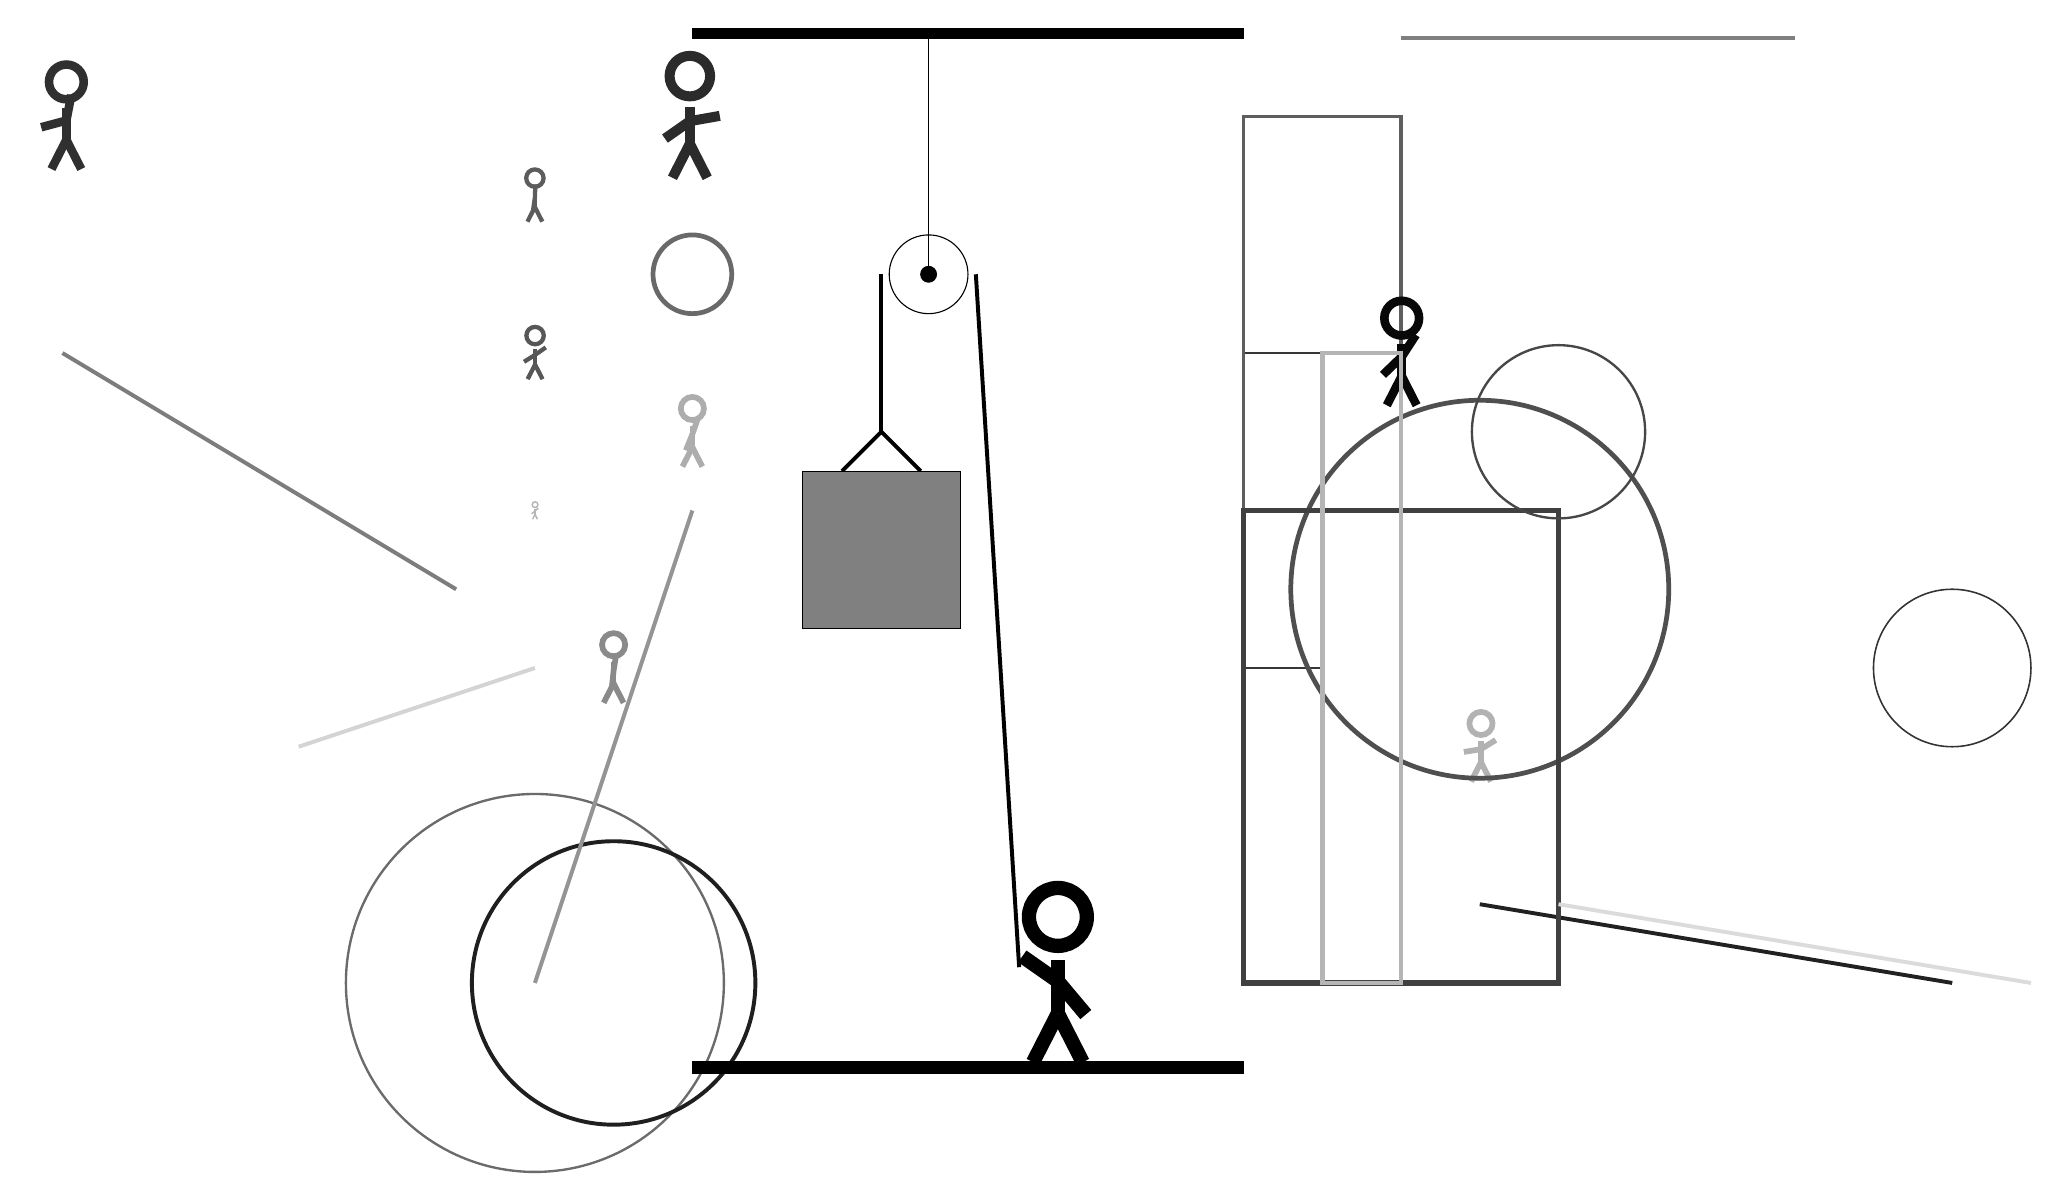
\begin{tikzpicture}
		%%%%% START %%%%%
		
		\draw[fill=black] (-2, 10) rectangle (5, 10.125);
		
		\draw (1, 7) circle (0.5);
		\draw[fill=black] (1, 7) circle (0.1);
		\draw (1, 10) -- (1, 7);
		
		\draw[line width=0.5mm] (-0.1, 4.5) -- (0.4, 5.0) -- (0.9, 4.5);
		\draw[fill=black!50] (-0.6, 4.5) rectangle (1.4, 2.5);
		
		\node[line width=0.7mm, color=black!83] at (-2, 9) {\Strichmaxerl[7][35][10]};
		
		\node[line width=0.3mm, color=black!30] at (8, 1) {\Strichmaxerl[4][9][32]};
		\draw[line width=0.5mm, color=black!87](8, -1) -- (14, -2);
		\node[line width=0.2mm, color=black!29] at (-4, 4) {\Strichmaxerl[1][38][44]};
		\draw[line width=0.2mm, color=black!79] (6, 6) rectangle (5, 2);
		\node[line width=0.7mm, color=black!46] at (-3, 2) {\Strichmaxerl[4][84][81]};
		
		\draw[line width=0.4mm, color=black!63] (7, 9) rectangle (5, -2);
		
		\draw[line width=0.5mm, color=black!50](7, 10) -- (12, 10);
		\draw [line width=0.6mm, color=black!69](8, 3) circle (2.4);
		\node[line width=0.6mm, color=black!97] at (7, 6) {\Strichmaxerl[6][44][57]};
		\draw[line width=0.7mm, color=black!75] (5, 4) rectangle (9, -2);
		
		\draw[line width=0.5mm, color=black!51](-5, 3) -- (-10, 6);
		\draw [line width=0.6mm, color=black!59](-2, 7) circle (0.5);
		
		\draw [line width=0.3mm, color=black!58](-4, -2) circle (2.4);
		\draw [line width=0.5mm, color=black!88](-3, -2) circle (1.8);
		\draw [line width=0.2mm, color=black!80](14, 2) circle (1.0);
		\draw[line width=0.5mm, color=black!42](-4, -2) -- (-2, 4);
		
		\node[line width=0.5mm, color=black!66] at (-4, 6) {\Strichmaxerl[3][32][35]};
		\node[line width=0.6mm, color=black!32] at (-2, 5) {\Strichmaxerl[4][68][71]};
		
		\node[line width=0.4mm, color=black!81] at (-10, 9) {\Strichmaxerl[6][15][79]};
		\draw [line width=0.3mm, color=black!72](9, 5) circle (1.1);
		
		\node[line width=0.6mm, color=black!64] at (-4, 8) {\Strichmaxerl[3][82][88]};
		\draw[line width=0.5mm, color=black!14](9, -1) -- (15, -2);
		\draw[line width=0.2mm, color=black!77] (6, 3) rectangle (6, 6);
		\draw[line width=0.6mm, color=black!29] (7, 6) rectangle (6, -2);
		
		\draw[line width=0.5mm, color=black!17](-7, 1) -- (-4, 2);
		
		\draw[line width=0.5mm] (0.4, 7) -- (0.4, 5.0);
		\centerarc[line width=0.5mm](1, 7)(0:180:0.6);
		\draw[line width=0.5mm](1.6, 7) -- (2.15, -1.8);
		
		\node at (2.6, -1.9) {\Strichmaxerl[10][-35][-50]};
		
		\draw[fill=black] (-2, -3) rectangle (5, -3.15);
		
		%%%%% END %%%%%
	\end{tikzpicture}
\end{document}